\documentclass[12pt]{article}

\usepackage{amsmath}
\usepackage[margin = 1in]{geometry}
\usepackage{graphicx}
\usepackage{booktabs}
\usepackage{natbib}

\usepackage{lipsum}
\usepackage[colorlinks=true, citecolor=blue]{hyperref}



\title{Stats Example Manuscript For STAT W}
\author{Miles Kee
}

\begin{document}
\maketitle

\begin{abstract}
This is the abstract. To fill some space, I'm going to paste in the lyrics to Shake It Off by Taylor Swift. I stay out too late Got nothing in my brain That's what people say That's what people say I go on too many dates But I can't make them stay At least that's what people say That's what people say But I keep cruising Can't stop, won't stop moving It's like I got this music in my mind Saying it's gonna be alright I never miss a beat I'm lightning on my feet And that's what they don't see That's what they don't see Players gonna play, play, play, play, play And the haters gonna hate, hate, hate, hate, hate (haters gonna hate) Baby, I'm just gonna shake, shake, shake, shake, shake I shake it off, I shake it off Heartbreakers gonna break Fakers gonna fake I'm just gonna shake I shake it off, I shake it off I shake it off, I shake it off I, I, I shake it off, I shake it off I, I, I shake it off, shake it off I, I, I shake it off, I shake it off I, I, I shake it off, I shake it off I, I, I shake it off, I shake it off I, I, I, shake it off, I shake it off I, I, I, shake it off, I shake it off
\end{abstract}

\section{Introduction}
\label{sec:intro}
In this section, I'm going to put some auto generated sentences in. Joe discovered that traffic cones make excellent megaphones. Random words in front of other random words create a random sentence. The best part of marriage is animal crackers with peanut butter. The sight of his goatee made me want to run and hide under my sister-in-law's bed. The most exciting eureka moment I've had was when I realized that the instructions on food packets were just guidelines. He decided water-skiing on a frozen lake wasn’t a good idea.

Gonna try to cite something now:
\citet{article1} talks about ... \lipsum[1].

Now, I am going to try to do a parenthetical citation \citep[][]{article2}.



%roadmap
The data will be included in Section~\ref{sec:data}.
The table will be in Section~\ref{sec:table}.
A discussion will be in Section~\ref{sec:discussion}.

\section{Data}
\label{sec:data}

Check out this cool equation!
\begin{equation}
  \label{eq:eq1}
  a^{2}=b^{2}+c^{2}.
\end{equation}
This sentence is to see what happens when I reference Equation~\ref{eq:eq1}.
\lipsum[1]

Equation~\ref{eq:eq2} shows the quadratic formula.
\begin{equation}
  \label{eq:eq2}
  x=\frac{-b\pm\sqrt{b^2-4ac}}{2a}.
\end{equation}

One other good equation is \(y=mx+b\), where can be rearranged into \(y-b=mx\).


\section{Table}
\label{sec:table}

Table~\ref{tab:sleep} shows how many hours of sleep I got this past week for each day.
\lipsum[1-4].

\begin{table}[tbp]
	\caption{Sleeping Table}
	\label{tab:sleep}
\centering
\begin{tabular}{rrr}
	\toprule
Day Of The Week & Sleep \\
	\midrule
Sunday & 7 \\
Monday & 6 \\
Tuesday & 6 \\
Wednesday & 4 \\
Thursday & 5 \\
	\bottomrule
\end{tabular}
\end{table}


\begin{figure}[tbp]
	\centering
	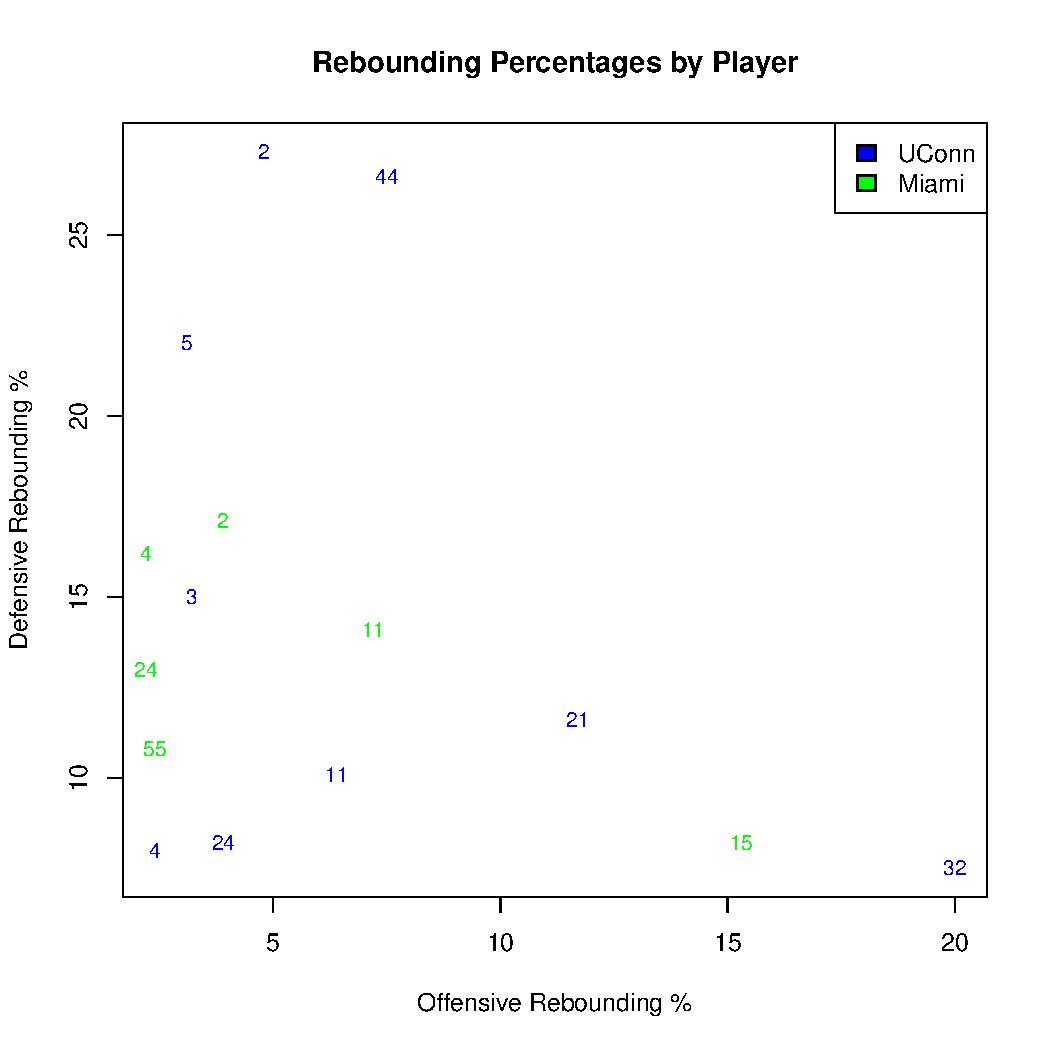
\includegraphics[width=\textwidth]{graph}
	\caption{A plot of UConn and UMiami's players offensive and defensive rebounding percentages.}
	\label{fig:graph}
\end{figure}

Figure~\ref{fig:graph} shows a graph I made to prepare for my interview with UConn Men's Basketball.


\section{Discussion}
\label{sec:discussion}

\lipsum[1-4].


\bibliography{workcited.bib}
\bibliographystyle{plainnat}



\end{document}